\documentclass[10pt]{article}
\usepackage[letterpaper]{geometry}
\geometry{verbose,tmargin=1in,bmargin=1in,lmargin=1in,rmargin=1in}
\usepackage{setspace}
\usepackage{ragged2e}
\usepackage{color}
\usepackage{titlesec}
\usepackage{graphicx}
\usepackage{float}
\usepackage{mathtools}
\usepackage{amsmath}
\usepackage[font=small,labelfont=bf,labelsep=period]{caption}
\usepackage[english]{babel}
\usepackage{indentfirst}
\usepackage{array}
\usepackage{makecell}
\usepackage[usenames,dvipsnames]{xcolor}
\usepackage{multirow}
\usepackage{tabularx}
\usepackage{arydshln}
\usepackage{caption}
\usepackage{subcaption}
\usepackage{xfrac}
\usepackage{etoolbox}
\usepackage{cite}
\usepackage{url}
\usepackage{dcolumn}
\usepackage{hyperref}
\usepackage{courier}
\usepackage{esvect}
\usepackage{commath}
\usepackage{verbatim} % for block comments
\usepackage{enumitem}
\usepackage{hyperref} % for clickable table of contents
\usepackage{braket}
\usepackage{titlesec}
\usepackage{booktabs}
\usepackage{gensymb}
\usepackage{listings}
\usepackage{cancel}
\usepackage[mathscr]{euscript}
\lstset{
    frame=single,
    	basicstyle=\ttfamily\small,
    breaklines=true,
    postbreak=\raisebox{0ex}[0ex][0ex]{\ensuremath{\color{red}\hookrightarrow\space}}
}

% for circled numbers
\usepackage{tikz}
\newcommand*\circled[1]{\tikz[baseline=(char.base)]{
            \node[shape=circle,draw,inner sep=2pt] (char) {#1};}}

\newcommand{\beq}{\begin{equation}}
\newcommand{\eeq}{\end{equation}}
\newcommand{\beqa}{\begin{equation}\begin{aligned}}
\newcommand{\eeqa}{\end{aligned}\end{equation}}

\titleclass{\subsubsubsection}{straight}[\subsection]

% define new command for triple sub sections
\newcounter{subsubsubsection}[subsubsection]
\renewcommand\thesubsubsubsection{\thesubsubsection.\arabic{subsubsubsection}}
\renewcommand\theparagraph{\thesubsubsubsection.\arabic{paragraph}} % optional; useful if paragraphs are to be numbered

\titleformat{\subsubsubsection}
  {\normalfont\normalsize\bfseries}{\thesubsubsubsection}{1em}{}
\titlespacing*{\subsubsubsection}
{0pt}{3.25ex plus 1ex minus .2ex}{1.5ex plus .2ex}

\makeatletter
\renewcommand\paragraph{\@startsection{paragraph}{5}{\z@}%
  {3.25ex \@plus1ex \@minus.2ex}%
  {-1em}%
  {\normalfont\normalsize\bfseries}}
\renewcommand\subparagraph{\@startsection{subparagraph}{6}{\parindent}%
  {3.25ex \@plus1ex \@minus .2ex}%
  {-1em}%
  {\normalfont\normalsize\bfseries}}
\def\toclevel@subsubsubsection{4}
\def\toclevel@paragraph{5}
\def\toclevel@paragraph{6}
\def\l@subsubsubsection{\@dottedtocline{4}{7em}{4em}}
\def\l@paragraph{\@dottedtocline{5}{10em}{5em}}
\def\l@subparagraph{\@dottedtocline{6}{14em}{6em}}
\makeatother


\setcounter{secnumdepth}{4}
\setcounter{tocdepth}{4}
\begin{document}

\title{MATH 228b: HW6}
\author{April Novak}

\maketitle

\section{}
The level set method propagates an implicit curve through a domain by solving a time-dependent convection equation, where the velocity in this equation is directly related to the physical processes that would move such a surface. Tracking the location of a surface is essential for numerical applications with moving boundaries, since the surface location must be known in order to apply boundary conditions correctly. For an implicit surface given by \(\phi(\vv{x})\), where \(\phi=0\) on the surface, \(\phi<0\) within the surface, and \(\phi>0\) outside, the convection equation that propagates the surface is:

\beq
\frac{\partial\phi}{\partial t}+\vv{V}\cdot\nabla\phi=0
\eeq

where \(\vv{V}\) is the speed of the surface. In physical applications, it is often the case that the velocity of the surface is in the normal direction \(\vv{n}\) of the curve, dictated by some speed function \(F\):

\beq
\vv{V}=F\vv{n}
\eeq

Inserting this speed into the convection equation gives the differential equation that propagates the implicit surface:

\beq
\frac{\partial\phi}{\partial t}+F|\nabla\phi|=0
\eeq

For cases where \(F\) is always positive, this initial value problem can be restated as a boundary value problem in terms of an arrival function \(T\), where \(T(\vv{x})\) represents the time for the interface to reach location \(\vv{x}\) from its initial location \(\Gamma\). This equation is:

\beq
|\nabla T|F=0
\eeq

where \(T=0\) on \(\Gamma\), since it takes zero time to arrive at the initial condition. Because \(T\) represents the time to reach the arrival point, \(T(x_{arrival}, y_{arrival})=t\). The level set with \(T=t\) represents the furthest point that can be reached in time \(t\) from the initial condition. Individual points move in the normal direction to these level sets, which allows this formulation to determine the optimal travel paths to the arrival location given an initial position. 

Instead of solving the above equation, we will use a time-dependent method that assumes that the solution will converge to the steady-state result in a sufficient number of iterations. Hence, we will solve:

\beq
\frac{\partial T}{\partial t}+|\nabla T|F=1
\eeq

for initial condition \(T(x_0, y_0)=0\), where \(x_0\) and \(y_0\) are on the initial curve \(\Gamma\). Integrating the above equation in time until steady-state is reached will give the solution to the Eikonal equation. A first-order upwinded scheme is used in space, and a simple forward Euler method in time. The initial condition for all cases is set to 0.0, and after every iteration, the sole boundary condition of \(\phi(0.2, 0.2)=0\) is strictly implied. A layer of ghost cells of a large value of \(\phi\) are inserted on the periphery in order to simplify the application of the one-sided upwind differencing. For this time-stepping solution, a time step of 0.0001 seconds is chosen, and appears sufficient.

Figures \ref{fig:case1} through \ref{fig:case4} show contours of the solution to \(\phi\) after reaching an iteration tolerance (defined based on successive differences in the infinity norm of \(\phi\) from one iteration to the next) of \(1e-10\) for the various cases given. The optimal path from the starting point and the given arrival point is calculated using a simple stepping scheme. Starting at the arrival point, a local gradient is computed using Matlab's {\tt interp2} function applied to the results of Matlab's {\tt gradient} function. The starting point is propagated for a small time step of {\tt 0.001} in the direction of this normal. After this short time, the gradient of this new location is re-computed, the point moved again, and the process continued until the point is within a distance of \(h\) from the starting point. The optimal paths are shown in the figures below as black lines, with the direction of travel beginning at \((0.2, 0.2)\) and ending at the given arrival point. As can be seen, the optimal path follows the local normal of \(\phi\), and reaches the starting point since this method is essentially a type of steepest-descent method. 

Case 4 places a square of width 0.2 centered on \((0.2, 0.2)\) and at \((0.6, 0.6)\), where the speed inside the square is 0.01 and outside is 1.0. Because the speed is so low through these two regions, the optimal path is to move around both squares, instead of taking the shortest-distance path through the centers of the squares.

\begin{figure}[H]
\centering
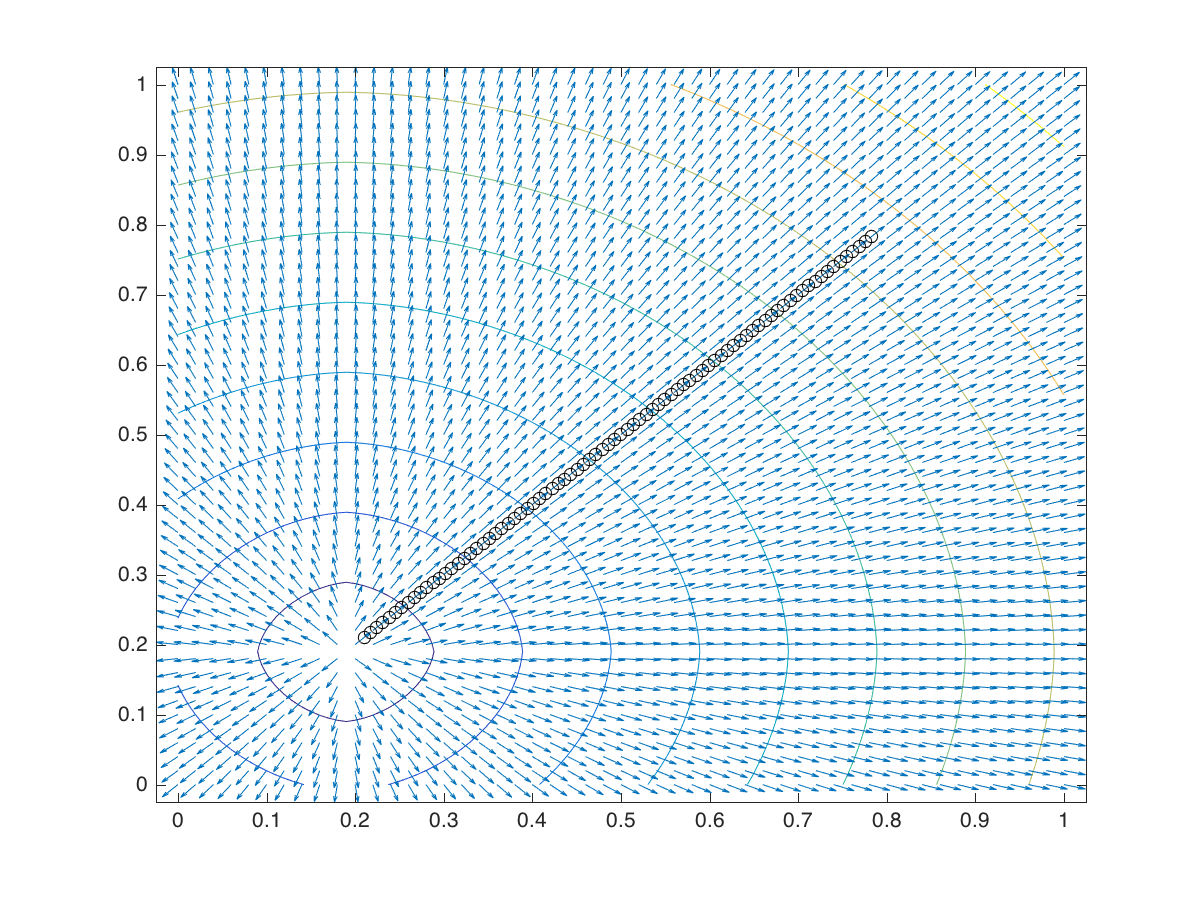
\includegraphics[width=0.8\textwidth]{figures/case1.png}
\caption{Contours of \(\phi(x, y)\) and the optimal travel path for case 1.}
\label{fig:case1}
\end{figure}

\begin{figure}[H]
\centering
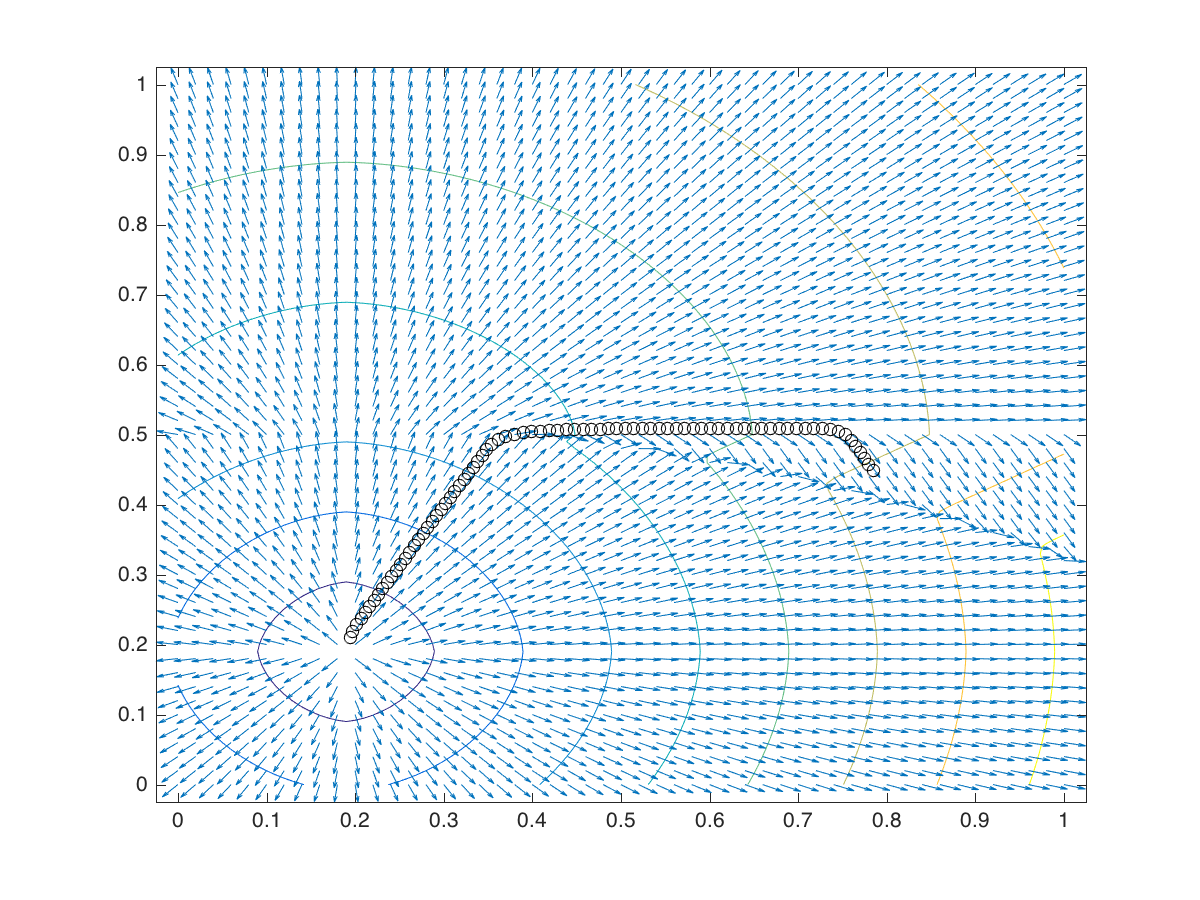
\includegraphics[width=0.8\textwidth]{figures/case2.png}
\caption{Contours of \(\phi(x, y)\) and the optimal travel path for case 2.}
\label{fig:case2}
\end{figure}

\begin{figure}[H]
\centering
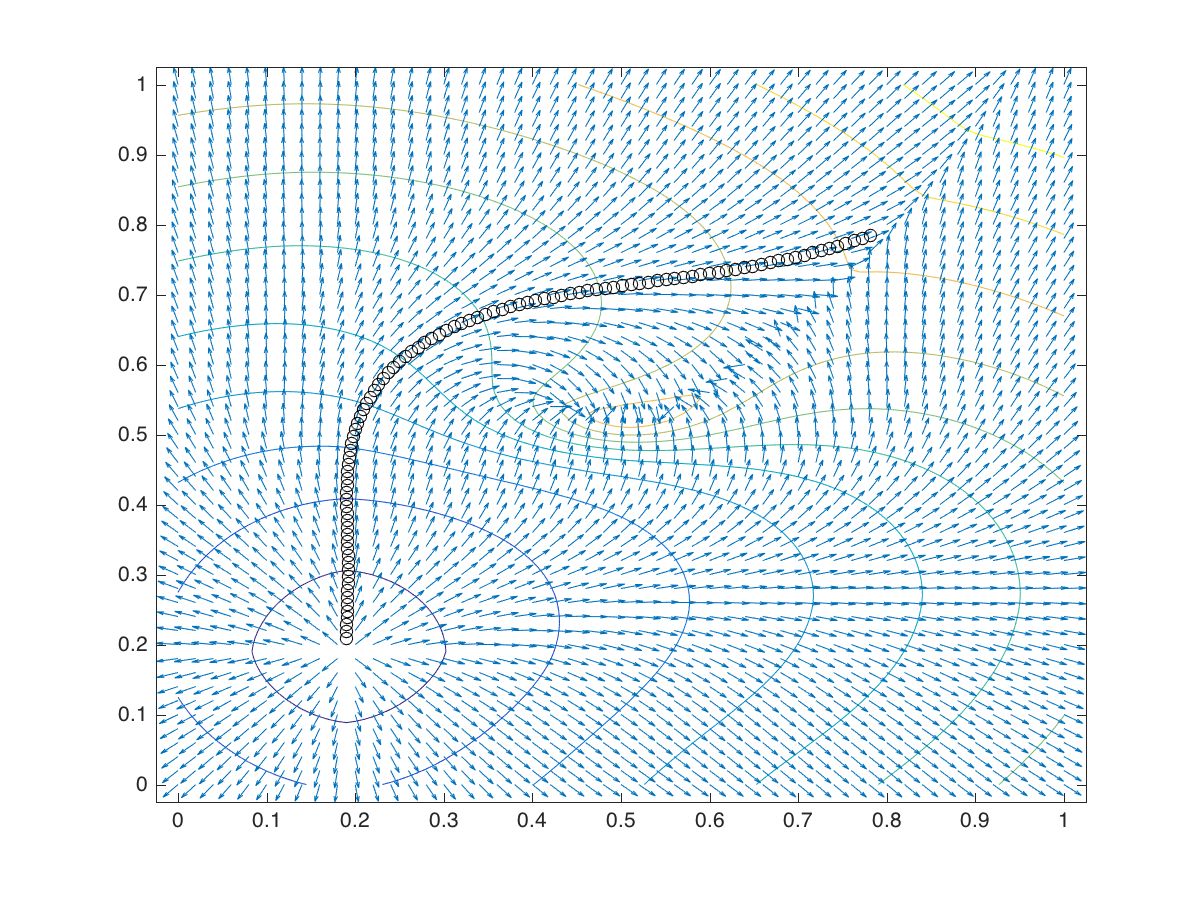
\includegraphics[width=0.8\textwidth]{figures/case3.png}
\caption{Contours of \(\phi(x, y)\) and the optimal travel path for case 3.}
\label{fig:case3}
\end{figure}

\begin{figure}[H]
\centering
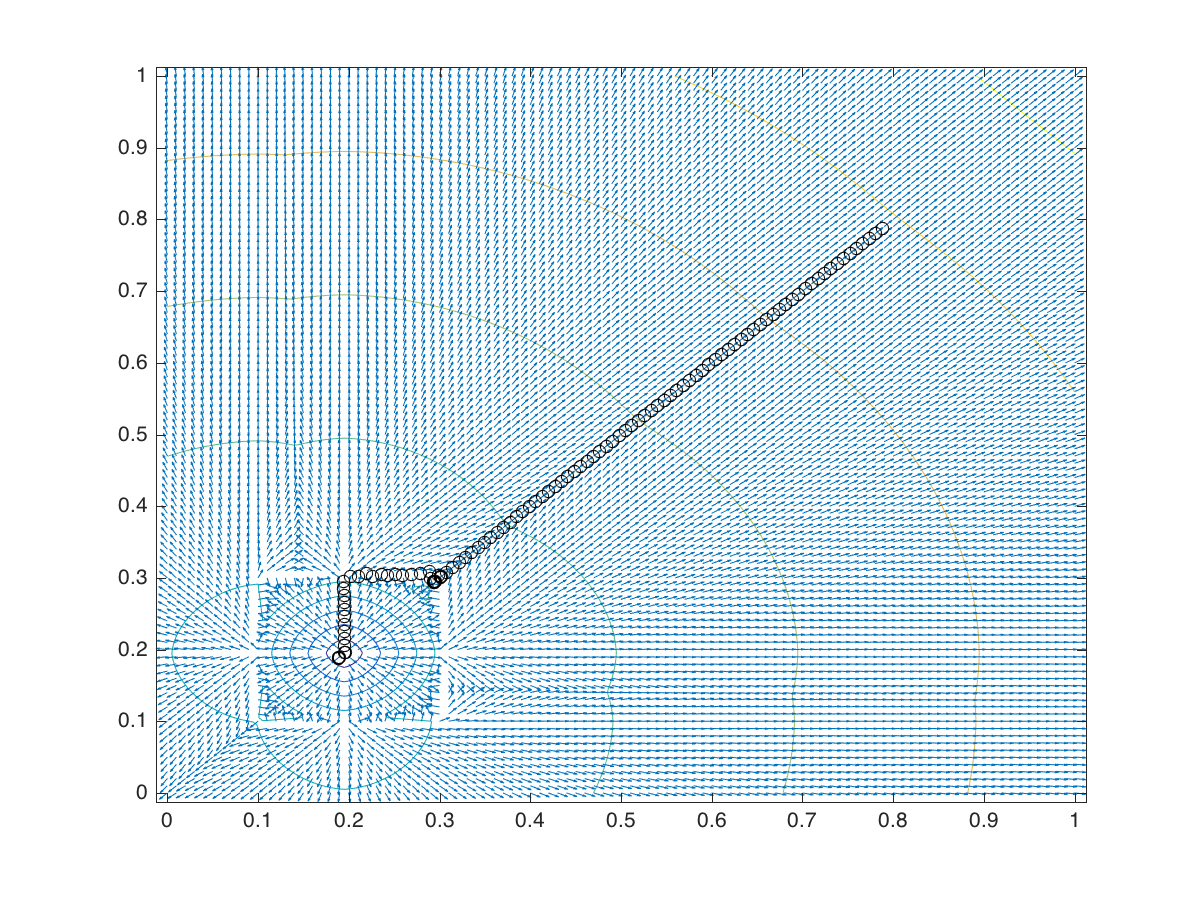
\includegraphics[width=0.8\textwidth]{figures/case4.png}
\caption{Contours of \(\phi(x, y)\) and the optimal travel path for case 4.}
\label{fig:case4}
\end{figure}

\section{}

\textbf{(a)}

The first part of this question develops a Gauss-Seidel solver given a matrix system \(Au=b\) for an initial guess \(u_0\). This method is very similar to the Jacobi method, where instead of solving the time-independent problem of interest, we insert a time derivative term and iterate until the solution converges to a steady-state result (with the assumption that this steady-state result is therefore also equivalent to the solution to the problem with no time derivative at all). Gauss-Seidel differs from the Jacobi method in that the most recent iterate is used to perform the update. The code developed for this section is included in the Appendix.

\textbf{(b)}

This question solves the Poisson equation using the multigrid method. The first step is a modification to Professor Persson's {\tt pmesh} function (which I assume is okay because we were told for assignment 3 that we could use his function moving forward to avoid points being lost across multiple assignments) such that it outputs the {\tt data} structured array data structure containing {\tt data.p}, {\tt data.t}, and {\tt data.e} members. This is performed by manipulating the contents of the original {\tt pmesh} function, so make sure to use the {\tt pmesh} function that I submit with this assignment! This edited function is included in the Appendix.

In order to simplify the multigrid method, which relies upon repeated applications of interpolation (expanding a coarse solution to a finer mesh) and reduction (removing elements from a solution to coarsen), these interpolation and reduction matrices are pre-computed. The matrices \(A\) and vectors \(b\) are then saved for the finest refinement level by running {\tt fempoi} only a single time, and then using the expansion and reduction matrices to project the finest matrix onto the coarser meshes.

\textbf{(c)}
The last part of this question solves the Poisson equation using the multigrid method, as shown in the {\tt mgsolve} function. A feature of the multigrid method is that the number of iterations required is independent of the mesh refinement. Convergence rates are shown in Fig. \ref{fig:question2c}, where it can indeed be seen that the number of iterations required to reach an infinity norm error of \(1e-10\) is roughly constant except for the coarsest mesh (and I'm not sure why that one converges faster). However, this is somewhat misleading, since the work per iteration does {\it not} stay constant with mesh spacing.

\begin{figure}[H]
\centering
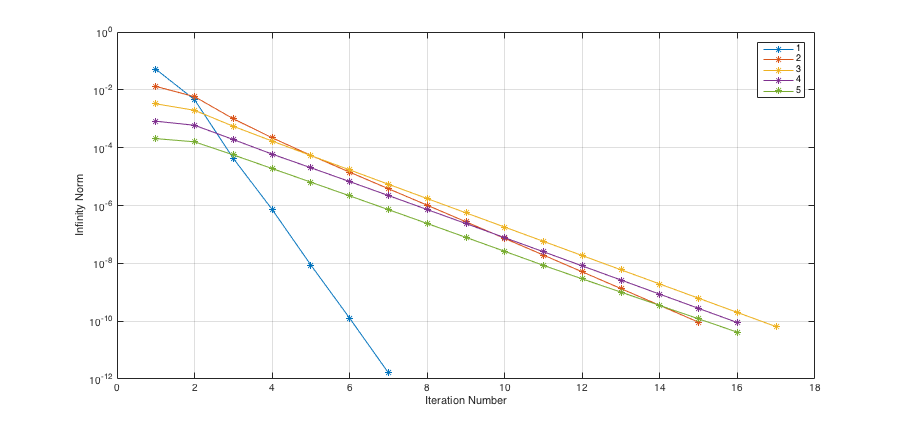
\includegraphics[width=1.0\textwidth]{figures/question2c.png}
\caption{Infinity norm as a function of iteration number for various refinement levels}
\label{fig:question2c}
\end{figure}










\section{Appendix}
\subsection{Question 1}
\subsubsection{{\tt eikonal.m}}
\lstinputlisting[language=Matlab]{eikonal.m}
\subsubsection{{\tt grad\_plus.m}}
\lstinputlisting[language=Matlab]{grad_plus.m}
\subsection{Question 2, part a}
\subsubsection{{\tt gauss\_seidel.m}}
\lstinputlisting[language=Matlab]{gauss_seidel.m}
\subsection{Question 2, part b}
\subsubsection{{\tt pmesh.m}}
\lstinputlisting[language=Matlab]{pmesh.m}
\subsubsection{{\tt mginit.m}}
\lstinputlisting[language=Matlab]{mginit.m}
\subsection{Question 2, part c}
\subsubsection{{\tt mgsolve.m}}
\lstinputlisting[language=Matlab]{mgsolve.m}

\end{document}
